\documentclass[10pt,a4paper]{article}

%double si on veut une version prof et une version élève. simple si on veut une seule version.
\newcommand{\buildmode}{double}

\InputIfFileExists{version.tex}{}{}
% Version (définie par le script)
\providecommand{\version}{eleve}

\usepackage{feuilleexo}

%%%à modifier à chaque fois

\renewcommand{\niveau}{1M}
\renewcommand{\chapitre}{Fonctions, généralités}
\renewcommand{\numchap}{0.1}
\renewcommand{\theme}{Fonctions}

\begin{document}




%\legendeicones

\vspace{-0.3cm}

\begin{prerequis}
\begin{itemize}
    \item Savoir lire une images, des antécédants, un ensemble de définition d'une fonction d'une fonction à partir de sa représentation graphique.
    \item Savoir tracer un tableau de signe et un tableau de variation d'un fonction à partir de sa représentation graphique.
\end{itemize}
\end{prerequis}

\begin{multicols}{2}

\section{Notations et calcul d'images}

\begin{exo}[Rappels][]
On considère une fonction \(f\) dont la représentation graphique est donnée ci-dessous.

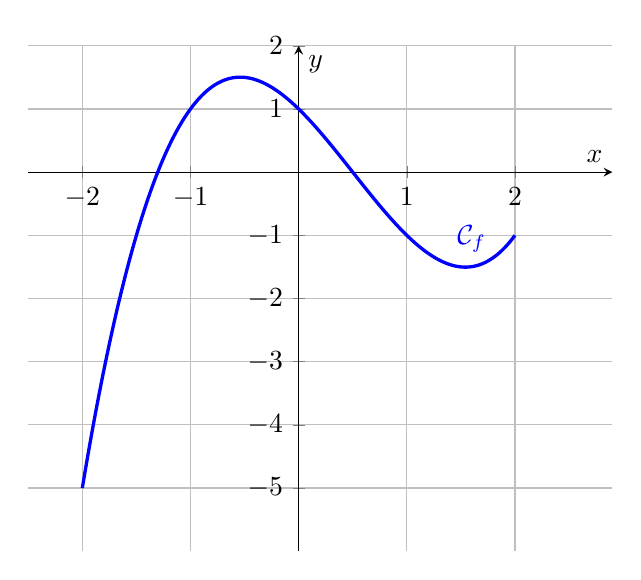
\begin{tikzpicture}
\begin{axis}[
    axis lines=middle,
    xmin=-2.5, xmax=2.9,
    ymin=-6, ymax=2,
    domain=-2:2,
    samples=300,
    grid=major,
    xtick={-2,-1,0,1,2,3},
    ytick={-5,-4,-3,-2,-1,0,1,2,3,4},
    xlabel={\(x\)},
    ylabel={\(y\)},
    width=9cm,
    height=8cm
]

\addplot[
    blue,
    very thick
] {2/3*(x-2)*(x+1.5)*(x-1)-1}
node[pos=0.92, above right] {\(\mathcal{C}_f\)};

\end{axis}
\end{tikzpicture}

\begin{enumerate}[leftmargin=*]
    \item Quel est l'ensemble de définition de \(f\) ?
    \item Donner les images de \(-2\), \(0\) et \(1\) par \(f\).
    \item Donner les éventuels antécédents de -1 et de 1.
    \item *Résoudre \(f(x)=0\).
    \item Établir le tableau de signes de \(f\) sur son ensemble de définition.
    \item Dresser le tableau de variations de \(f\) sur son ensemble de définition.
\end{enumerate}
\end{exo}

\prof{\begin{enumerate}
    \item verbaliser une première fois les informations codées par un tableau de signe et de un tableau de variation.
\end{enumerate}
    }

\begin{exo}[][]
On considère une fonction \(g\) dont la représentation graphique est donnée ci-dessous.

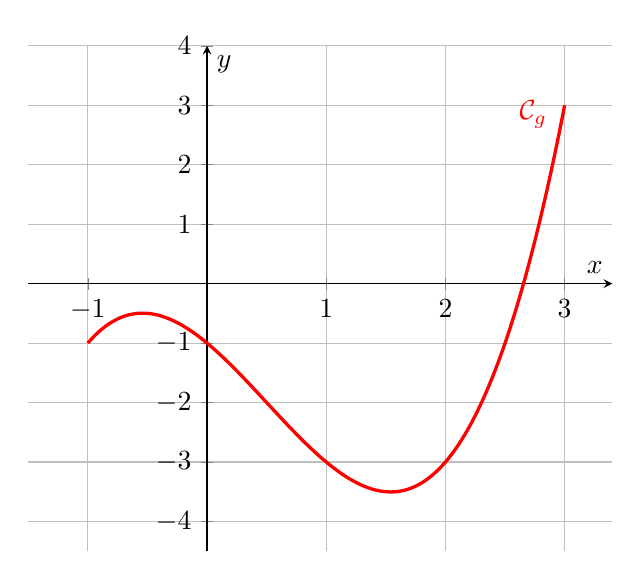
\begin{tikzpicture}
\begin{axis}[
    axis lines=middle,
    xmin=-1.5, xmax=3.4,
    ymin=-4.5, ymax=4,
    domain=-1:3,
    samples=300,
    grid=major,
    xtick={-2,-1,0,1,2,3,4},
    ytick={-4,-3,-2,-1,0,1,2,3,4},
    xlabel={\(x\)},
    ylabel={\(y\)},
    width=9cm,
    height=8cm
]

\addplot[
    red,
    very thick
] {2/3*(x+1)*(x-2.5)*(x)-1}
node[pos=0.95, above left] {\(\mathcal{C}_g\)};

\end{axis}
\end{tikzpicture}

\begin{enumerate}[leftmargin=*]
    \item Quel est l'ensemble de définition de \(g\) ?
    \item Donner les images de \(-1\), \(0\) et \(2\) par \(g\).
    \item Donner les éventuels antécédents de \(-3\) et de \(-1\).
    \item *Résoudre \(g(x)=0\).
    \item Établir le tableau de signes de \(g\) sur son ensemble de définition.
    \item Dresser le tableau de variations de \(g\) sur son ensemble de définition.
\end{enumerate}
\end{exo}

\prof{
    Même objectif que l'exercice précédent, avec une courbe présentant deux extremums locaux : bonne occasion de vérifier que la lecture du tableau de variations est acquise avant de passer aux exercices \og appro \fg{}.
}

\begin{exo}[][appro]
    
On donne le tableau de signe suivant :

\begin{center}
\begin{tikzpicture}
\tkzTabInit[lgt=1.1,espcl=1.3]{\(x\) /1, \(f(x)\) /1}{\(-4\),\(-2\),\(1\),\(3\),\(5\)}
\tkzTabLine{,+,0,-,0,+,0,-,}
\end{tikzpicture}
\end{center}

Tracer une fonction admettant ce tableau de signes.
\end{exo}

\prof{
    Faire verbaliser le tableau de signes par les élèves et le tableau de variations.
}

\begin{exo}[][appro]
On donne le tableau de variations suivant :

\begin{center}
\begin{tikzpicture}
\tkzTabInit[lgt=1.1,espcl=1.3]{\(x\) /1, \(f\) /2}{\(-4\),\(0\),\(4\),\(5\)}
\tkzTabVar{+/\(4\),-/\(-2\),+/\(6\),-/\(-2\)}
\end{tikzpicture}
\end{center}

Tracer une fonction admettant ce tableau de variations.
\end{exo}

\begin{exo}[][avance]
    Est-il possible de tracer une fonction ayant pour tableaux de signe et de variations les deux tableaux ci-dessus ? Justifier.
\end{exo}

\prof{
    Contradiction non évidente pour des élèves en début de première. Plusieurs méthodes possibles :
   
   \smallskip

    - Remarquer que la valeur en 4 est négative dans le premier tableau et positive dans le 2e.

    \smallskip
    
    - Approche intuitive du TVI.
}

\end{multicols}

\end{document}
